% ------------------------------------------------
% *** Section 1: Introduction ***
% ------------------------------------------------
\newpage
\chapter{Introduction}
\section{Getting Started}
% Perhaps, move this block after building and running AstraKernel subsection
AstraKernel begins its life in a small bootstrap routine, written in ARM assembly, 
that prepares the processor’s state before passing control to the main C kernel. 
This bootstrap code is responsible for setting up the stack pointer, clearing 
the uninitialized data section (\texttt{.bss}), and ensuring a clean environment 
for the kernel’s entry point. Below is the initial assembly code that executes 
at startup: \\

\begin{lstlisting}[language={C}, caption={Initial bootstrap code for AstraKernel.}, label={lst:bootstrap}]
    .section .text
    .global _start

_start:
    // Set up the stack pointer
    LDR sp, =_estack
    BIC sp, sp, #7
    // Zero the .bss section
    LDR R0, =__bss_start   // Start address (symbol from linker script)
    LDR R1, =__bss_end     // End address (symbol from linker script)
    MOV R2, #0             // init zero-value for BSS clearing

zero_bss:
    // Check if we are done zeroing the BSS
    CMP R0, R1             // Compare current address to end
    BGE bss_done           // If done, skip zeroing
    STR R2, [R0], #4       // Store zero at [r0], increment r0 by 4
    B zero_bss

bss_done:
    // Call kernel_main function
    BL kernel_main

hang:
    // Halt if kernel_main returns (should not happen)
    B hang		// Infinite loop
\end{lstlisting}

This startup sequence is the essential first step for any kernel, ensuring the 
CPU is properly initialized and memory is in a known state before higher-level 
code takes over. Once these preparations are complete, the \texttt{kernel\_main} 
function from \texttt{kernel/kernel.c} is called, marking the transition from 
low-level assembly to the C code that forms the core of AstraKernel.

% TODO: Explain the assembly code in more detail, specifically the
% stack pointer setup and BSS clearing process.

\subsection{Prerequisites}

Before you can build and run AstraKernel, please ensure you have the following 
tools installed on your system:

\begin{itemize}
  \item \textbf{ARM Cross-Compiler:}  
  A cross-compiler targeting ARM is required to build the kernel. It 
  is recommended to use \texttt{arm-none-eabi-gcc}, \texttt{arm-none-eabi-ld}, 
  and \texttt{arm-none-eabi-objcopy} for ARM926EJ-S, which is the target architecture
  for AstraKernel.
  \begin{itemize}
    \item Example installation: \texttt{arm-none-eabi-xxx} (available via package 
    managers such as \texttt{brew}, \texttt{apt}, or direct download from ARM's website).
  \end{itemize}
  
  \item \textbf{QEMU Emulator:}  
  QEMU is used to emulate the ARM VersatilePB (ARM926EJ-S) platform for kernel development and testing.
  \begin{itemize}
    \item Ensure your QEMU installation supports the \texttt{versatilepb} machine.
    \item Example installation: \texttt{qemu-system-arm} via  qemu \url{https://www.qemu.org/download/}.
  \end{itemize}

  \item \textbf{Build Tools:}  
  Standard build tools such as \texttt{make} are required to compile the kernel.
  \begin{itemize}
    \item Example installation: \texttt{make} (available via package managers 
    such as \texttt{brew}, \texttt{apt}, or direct download \url{https://www.gnu.org/software/make/#download}).
  \end{itemize}
\end{itemize}

\noindent
For best results, ensure all tools are up-to-date. Consult the official documentation 
of each tool for installation instructions on your operating system.

\subsection{Building \& Running AstraKernel}

\begin{note}
  The following instructions assume you have the necessary tools installed on your 
  system as mentioned in the prerequisites.
\end{note}

This project uses \texttt{Make} to automate the build process. The configuration
is located in the \texttt{Makefile} in the root directory of the kernel source code.
To build and run the kernel, navigate to the root directory of the AstraKernel source code
and execute the following command in your terminal: \\

\begin{lstlisting}[language={bash}, caption={Building AstraKernel.}, label={lst:build}]
make
\end{lstlisting}

\noindent
This command invokes the Makefile, which automatically compiles the kernel 
source code, links the object files, and generates the final kernel binary. The 
output files are placed in the \texttt{build/} directory, and any previously 
compiled files there are removed to ensure a clean build environment. Finally, 
the commands also run \texttt{make qemu}, which launches the QEMU emulator with the 
built kernel image. \\

\begin{lstlisting}[language={make}, caption={Makefile for AstraKernel.}, label={lst:makefile}]
  # Assembly start.o goes to build/
  $(OUT_DIR)start.o: kernel/start.S
    @mkdir -p $(OUT_DIR)
    $(AS) -c $< -o $@

  # Pattern rule for any .c -> build/*.o
  $(OUT_DIR)%.o: %.c
    @mkdir -p $(OUT_DIR)
    $(CC) $(CFLAGS) -c $< -o $@

  # Link everything
  $(OUT_DIR)kernel.elf: $(OUT_DIR)start.o $(OBJS) kernel.ld
    $(LD) $(LDFLAGS) $(OUT_DIR)start.o $(OBJS) -o $@

  # Generate the kernel binary from the ELF file
  kernel.bin: $(OUT_DIR)kernel.elf
    $(OBJCOPY) -O binary $< $(OUT_DIR)$@
\end{lstlisting}

\begin{info}
  You can run each \texttt{make} target on its own. Run \texttt{make kernel.bin} 
  to compile the kernel binary, \texttt{make qemu} to launch the built kernel in 
  QEMU, and \texttt{make clean} to remove all object files and the \texttt{kernel.bin} 
  from the \texttt{build/} directory.
\end{info}

\noindent
If the build is successful, you will see the output similar to the following:

\begin{figure}[H]
  \centering
  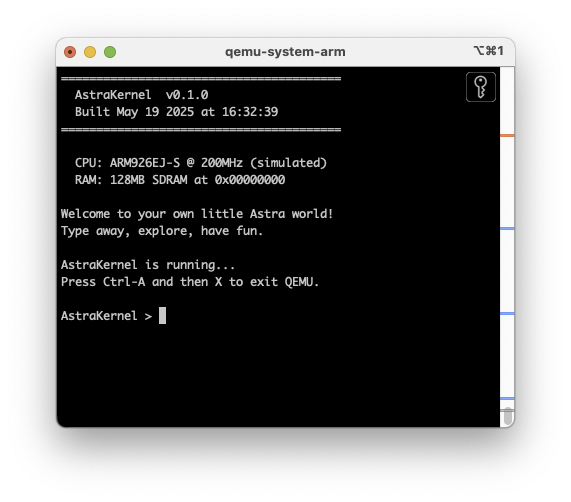
\includegraphics[width=0.5\textwidth]{figures/bootedKernel.png}
  \caption{AstraKernel booted in QEMU.}
  \label{fig:bootedKernel}
\end{figure}
